\chapter{Photo-nuclear interactions \label{ch:photoNuc}}
    In ultra-peripheral heavy-ion collision, the colliding nuclei interact only 
      electromagnetically~\cite{Baltz:2007kq,Bertulani:2005ru}.   
    In such events, no QGP state emerges, and the effects arising from the QGP 
      no longer obscure the initial state effects.
    Other initial state probes such as peripheral nuclear collisions and 
      proton-nucleus collisions have the potential to create the QGP obscuring 
      which effects come from the initial state.
    In UPC events the nuclei do not collide, therefore final state effects coming
      from the QGP are not expected. 
    Thus, UPC events provide clarity by enhancing physicists' 
      understanding of the initial state. 
    
    In particular, these interactions between the field of photons surrounding 
      the colliding nuclei and the gluons within the nuclei can produce a 
      \JPsi{}, probing the gluon density~\cite{Ryskin:1992ui,Brodsky:1994kf}.
    The \JPsi{} can be produced either coherently or incoherently. 
    In the case of coherent interactions, the photon couples to the nucleus 
      as a whole.
    In the incoherent case, the photon couples to the nucleons within the 
      nucleus.
    The UPC \JPsi{} photoproduction cross section is therefore a probe of 
      the initial state of the nucleus.

    This cross section can be calculated using three steps.   
    First, the Weizs\"{a}cker-Williams approximation~\cite{vonWeizsacker:1934sx,Williams:1934ad} provides a way to calculate the 
      density of probing photons that surrounds the nucleus. 
    Second, the electron-proton scattering data gives a value for the proton 
      photoproduction cross section at lower energies \cite{Klasen:2007pm}.
    Last, a specific model is used to combined the previous two steps in order
      to calculate the nuclear photoproduction cross section. 
    In this thesis the Adeluyi and Bertulani (AB)~\cite{pQCD2011.08,pQCD2013.02}, STARlight~\cite{vmd1999,starlight}, and 
      the Leading Twist (LTA)~\cite{Frankfurt:2011cs,lta2011.09} models are discussed. 
    Each of these methods handle the gluon density of the nucleus differently 
      producing a measurable difference in the value of the \JPsi{} 
      photoproduction cross section. There are other UPC models available~\cite{Goncalves:2011vf,Cisek:2012yt,Lappi:2013am,Hufner:1996jw}, but this thesis focuses on the three models mentioned because 
STARlight is the Monte Carlo generator used throughout this analysis, while the other two are models are the ones that show the best agreement 
with previous measurements by the ALICE Collaboration~\cite{Abelev:2012ba,Abbas:2013oua}. 
They have provided important constrains to models of the nuclear gluon density~\cite{lta2013.05}.
    The analysis presented in Chapter~\ref{ch:analysis} adds to the existing 
      data in a new kinematic region.
    In this Chapter the theoretical framework for photon-nuclear
      interactions, together with an experimental review of recent results on 
      ultra-peripheral heavy-ion collisions are described. 

  \section{Weizs\"{a}cker-Williams approximation \label{sec:wwAprox}}
    The density of photons surrounding the colliding nuclei can be calculated 
      using the Weizs\"{a}cker-Williams approximation~\cite{vonWeizsacker:1934sx,Williams:1934ad}. 
    This approximation relates the electric field of a stationary point charge 
      to the photon field that arises at ultra relativistic velocities. 
    The approximation is semi-classical and combines both classical and quantum 
      elements.
    In the Weizs\"{a}cker-Williams 
      approximation, a Fourier transform of Maxwell's equations is combined 
      with the quantum mechanical equation for the energy of the photon.   
    \begin{figure}[!Hhbt]
      \begin{center}
        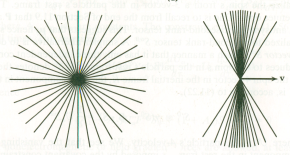
\includegraphics[width=.65\textwidth]{boost.png}
      \end{center}
      \caption{ \label{fig:boost} The electromagnetic field boosted and at rest. }
    \end{figure}
    The frequency modes of the electrostatic field are treated as photons. 
    The Weizs\"{a}cker-Williams approximation makes the calculation of 
      electromagnetic interactions with the nucleus tractable. 

    The Weizs\"{a}cker-Williams approximation begins with the equation for the 
      electric field of the projectile nucleus at rest. 
    To calculate the photon flux on the target nucleus, the electromagnetic field 
      only needs to be considered at the position of the target nucleus. 
    From the projectile's point of view, the target is moving and contributes
     $-vt$ to Eq.~\ref{eq:staticEFromTargtmp}, the equation for the electric 
     field of the projectile nucleus at rest.
    \begin{equation} \label{eq:staticEFromTargtmp}
        x'=-vt'\textrm{,}\qquad
        y'=b\textrm{,}\qquad
        z'=0\textrm{,}\qquad
        \vec{\mathbf{E'}}=\left(\frac{eZ}
         {4 \pi \epsilon_{0}\left(\left(-vt'\right)^{2}+b^{2}\right)^{3/2}}\right)
         \left(-vt'{\mathbf{\hat{x'}}+b\mathbf{\hat{y'}}}\right)\textrm{,}
    \end{equation}        
      where $b$ is the impact parameter
      defined as the distance of separation at closest approach, $v$ is the velocity of the 
      projectile nucleus, $Z$ is the number of protons in the nucleus, and $e$ 
      is the charge of the electron.
    Two simplifications occur due to the choice of coordinates in 
      Eq.~\ref{eq:staticEFromTargtmp}.
    The magnetic field is equal to zero, as the projectile is at rest, and
      the $z$ coordinate can be ignored, reducing the equation to two dimensions. 

    The Lorentz transformation converts the field equations in the 
      projectile's frame to equations in the target's frame.
    Eq.~\ref{eq:staticEFromTarg2tmp} gives the result of the transformation 
      from the projectile's primed frame to the target's rest frame for 
      the field components \cite{WWJackson}:
    \begin{eqnarray} \label{eq:staticEFromTarg2tmp}
        E_{x}'=E_{x}\textrm{,}\qquad
        \gamma\left(E_{y}'/c+\beta B_{z}'\right)=E_{y}/c\textrm{,}\qquad
        \gamma\left(E_{z}'/c=\beta B_{y}'\right)=E_{z}/c\textrm{,} \nonumber \\
        B_{x}'=B_{x}\textrm{,}\qquad
        \gamma\left(B_{y}'-\beta E_{z}'/c\right)=B_{y}\textrm{, and}\qquad
        \gamma\left(B_{z}'+\beta E_{y}'/c\right)=B_{z}\textrm{.}
    \end{eqnarray}
    The transformation equations for the fields, 
      Eq.~\ref{eq:staticEFromTarg2tmp}, and the transformation of the 
      coordinates reduce to Eq.~\ref{eq:staticEFromTarg3tmp} \cite{WWJackson}:
    \begin{eqnarray} \label{eq:staticEFromTarg3tmp}
        E_{x}'=E_{x}\textrm{,}\qquad
        \gamma E_{y}'=E_{y}\textrm{,}\qquad
        \gamma \beta E_{y}'/c=B_{z}\textrm{,}\nonumber \\
        ct'=\gamma ct\textrm{, and}\qquad
        x'=-\gamma \beta c t\textrm{.}
    \end{eqnarray}
    The Lorentz transformation reduces the six components of the 
      electromagnetic field in the target's frame to the three equations in 
      Eq.~\ref{eq:staticEFromTarg2tmp} by relating them to the fields in the 
      projectile's frame. 
    
    By combining Eq.~\ref{eq:staticEFromTargtmp} and 
      Eq.~\ref{eq:staticEFromTarg2tmp}, equations for the electric and 
      magnetic fields in the target's rest frame are obtained 
        \begin{eqnarray} \label{eq:ebPframe} 
          \vec{\mathbf{E}}=\left( \frac{\gamma e Z}
           { 4 \pi \epsilon_{0} \left( \left( \gamma v t \right)^{2} 
           + b^{2}\right)^{3/2} }\right)
           \left(vt\mathbf{\hat{x}}+b\mathbf{\hat{y}}\right)\nonumber\textrm{, and} \\
           \vec{\mathbf{B}}=\frac{\gamma\beta e Z b}
           { 4 \pi c \epsilon_{0} \left( \left( \gamma v t \right)^{2} 
           + b^{2}\right)^{3/2} }
           \mathbf{\hat{z}}=
           \frac{\gamma\mu_{0}veZb}{4\pi\left(\left(\gamma v t \right)^{2}
           +b^{2}\right)^{3/2}}\mathbf{\hat{z}}.
        \end{eqnarray}
    If the impact parameter $b$ goes to zero, the target sits in the line of 
      the projectile particle's motion, and the denominator carries a factor of
      $\gamma$ squared. 
    When $vt$ goes to zero, the projectile particle position lays on the 
      $y$-axis, and the numerator carries a factor of $\gamma$. 
    This results in fields that are a factor of $\gamma^3$ higher in the 
      $y$ direction than in the $x$ direction (see Fig.~\ref{fig:boost}).  
    The boost compresses the electric field of the charge 
      in the direction of the boost and produces a magnetic field 
      resulting in a form similar to radiation.
    The point charge at ultra relativistic velocities produces a strong 
      electric field in the plane transverse to its motion resembling a plane 
      wave.
         
    Separating the electromagnetic field into even and odd functions of time 
      simplifies the decomposition of the field equations into Fourier frequency 
      modes.
    The even functions decompose into cosine functions, odd functions 
      into sine functions. 
    The $y$-component of the electric field and the $z$-component of 
      the magnetic field are even functions in time, and the 
      $x$-component of the electric field is an odd function in time.
    Eq.~\ref{eq:fourier1tmp} gives the Fourier transformation integrals. 
    \begin{eqnarray} \label{eq:fourier1tmp}
        E_{x}(\omega)=\sqrt{\frac{2}{\pi}}\frac{eZ}{4\pi\epsilon_{0}b^{2}}
         \int^{\infty}_{0}\frac{\left(\gamma vt/b\right)\sin
         \left(\omega t\right)}
         {\left(\left(\gamma vt/b\right)^{2}+1\right)^{3/2}}dt\textrm{,} \nonumber\\
          E_{y}(\omega)=\sqrt{\frac{2}{\pi}}\frac{\gamma eZ}
         {4\pi\epsilon_{0}b^{2}} \int^{\infty}_{0}\frac{\cos(\omega t)}
         {\left(\left(\gamma vt/b\right)^{2}+1\right)^{3/2}}dt\textrm{,  and}\\
          B_{z}(\omega)=\frac{\beta E_{y}(\omega)}{c}.\nonumber
    \end{eqnarray}
    The solutions to the integrals of Eq.~\ref{eq:fourier1tmp} are the following
      \cite{WWFermi}:
    \begin{eqnarray}  \label{eq:fourier2tmp}
      u=\frac{\gamma v t}{b}\textrm{,}\qquad du\left(\frac{b}{\gamma v}\right)=dt\textrm{,}\qquad
      \omega'=\frac{\omega b}{\gamma v}\textrm{,}\nonumber \\
      \int^{\infty}_{0}\frac{u \sin(\omega'u)}{\left(u^{2}+1\right)^{3/2}}du
      =\omega'K_{0}(\omega')\textrm{, and}\qquad
      \int^{\infty}_{0}\frac{\cos(\omega'u)}{\left(u^{2}+1\right)^{3/2}}
      =\omega'K_{1}(\omega').
    \end{eqnarray}
    In Eq.~\ref{eq:fourier2tmp}, $\omega$ can be related to the energy of a 
      photon by $E=\hbar\omega$.
    The components of the electric field in terms of $\omega$ are:
    \begin{equation} \label{eq:fourier3tmp}
        E_{x}(\omega)=\sqrt{\frac{2}{\pi}}\frac{eZ}{4\pi\epsilon_{0}b^{2}}
     \frac{b}{\gamma v}\frac{\omega b}{\gamma v}K_{0}
     \left(\frac{\omega b}{\gamma v}\right)\textrm{, and}\qquad
      E_{y}(\omega)=\sqrt{\frac{2}{\pi}}\frac{\gamma eZ}{4\pi\epsilon_{0}b^{2}}
     \frac{b}{\gamma v}\frac{\omega b}{\gamma v}K_{1}
     \left(\frac{\omega b}{\gamma v}\right).\qquad
    \end{equation}
    The $y$-component of the electric field does not have a factor of $t$ in 
      the numerator in Eq.~\ref{eq:fourier1tmp}, therefore the factor of $\gamma$ 
      remains outside of the integral for the Bessel functions in 
      Eq.~\ref{eq:fourier3tmp}.
    In Eq.~\ref{eq:fourier3tmp}, $E_{y}$ carries an additional factor of 
      $\gamma$ in the numerator relative to the $E_{x}$, therefore in the case
      when $\gamma >> 1$, $E_{x}$ can be neglected. 

    When $v$ approaches $c$, $\beta \approx 1$, the $y$-component of the 
      electric field and the $z$-component of the magnetic field are related by 
      a factor of $c$, $E_{y}/c=B_{z}$.
    $E_{y}$ is approximately equally to $\gamma$ $E_{x}$ because $K_{0}(x)$ is 
      smaller than $K_{1}(x)$ for all $x$. 
    The conditions imposed by the ultra-relativistic limit result in the 
      following relationship
    \begin{equation} \label{eq:ultraRelAprox}
      \gamma \gg 1 \Rightarrow \gamma E_{x} \gg E_{x} \Rightarrow E_{y} \gg E_{x} \textrm{.}
    \end{equation}
    The six field components are reduced to one electric component and one 
      perpendicular magnetic field component, which have a configuration 
      identical to a plane wave. 

    As with plane waves, the energy per area per time transferred by 
      the electromagnetic field is given by the Poynting vector.
    The Poynting vector takes the simple form of a plane pulse propagating in 
     the $x$ direction as given by
    \begin{equation} \label{eq:poyntingVectortmp}
        \vec{\mathbf{S}}\equiv
        \vec{\mathbf{E}}\times\vec{\mathbf{B}}/\mu_{0}=
        \left(E_{y}^{2}/c\mu_{0}\right)\mathbf{\hat{x}}=
        c\epsilon_{0}E_{y}^{2}\mathbf{\hat{x}}.
    \end{equation}
    The Poynting vector relates to the fluence (energy per unit area) 
      by the expression \cite{WWBrau} 
    \begin{equation} \label{eq:fluencytmp}
        I(b)=\mathbf{\hat{x}}\cdot\int^{\infty}_{0}\vec{\mathbf{S}}d\omega=
         \int^{\infty}_{0}\left(c\epsilon_{0}E_{y}^{2}\right)d\omega=
         \int^{\infty}_{0}\left(\frac{dI}{d\omega}\right)d\omega,
    \end{equation}
      and the spectral fluence (energy per area per frequency) is given 
      by
    \begin{equation} \label{eq:specturalFluencytmp}
      \frac{dI}{d\omega}=c\epsilon_{0}E_{y}^{2}=
       \frac{e^{2}Z^{2}c}{4\pi^{3}b^{2}v^{2}\epsilon_{0}}
       \left(\frac{\omega b}{\gamma v}\right)^{2}
         K_{1}^{2}\left(\frac{\omega b}{\gamma v}\right)=
        \alpha\hbar\left(\frac{Z}{b\beta\pi}\right)^{2}
         \left(\frac{\omega b}{\gamma v}\right)^{2}
       K_{1}^{2}\left(\frac{\omega b}{\gamma v}\right).
    \end{equation}
    The spectral fluence given by Eq.~\ref{eq:specturalFluencytmp} 
      relates the frequency to energy. 
    The quantum mechanical equation, $E=\hbar\omega$, gives the energy of a 
      photon, which is related to the spectral fluence. 
    The relationship between the photon number density and the spectral fluence
      is \cite{WWJackson}
    \begin{equation}  \label{eq:photonFluxtmp}
        \frac{dI}{d\omega}d\omega=\hbar\omega N(\omega)d(\hbar\omega)
        \Rightarrow \frac{1}{\hbar^{2}\omega}\frac{dI}{d\omega}=N(\omega).
    \end{equation}
    Substituting Eq.~\ref{eq:specturalFluencytmp} into 
      Eq.~\ref{eq:photonFluxtmp} yields the semiclassical photon flux:
    \begin{equation} \label{eq:photonFluxFinaltmp}
      N(\omega,b)=\frac{\alpha}{\hbar\omega}
       \left(\frac{Z}{b\beta\pi}\right)^{2}
       \left(\frac{\omega b}{\gamma v}\right)^{2}
       K_{1}^{2}\left(\frac{\omega b}{\gamma v}\right).
    \end{equation}
    This replaces the classical electric field of a point charge with a 
      semiclassical field of photons. 
    The photon flux in Eq.~\ref{eq:photonFluxFinaltmp} provides the 
      electromagnetic input to the \JPsi{} photoproduction cross section 
      calculation. 

  \section{\label{sec:vdmTheory}The STARlight model}
    The STARlight model~\cite{vmd1999,starlight} for calculating the \JPsi{}
      photoproduction cross section has three main components.
    The STARlight approach is constructed from the Weizs\"{a}cker-Williams 
      photon flux, uses the vector meson dominance fit to the proton-electron data, 
      and uses the Glauber model~\cite{Miller:2007ri} for calculating the nuclear cross sections from 
      the proton-electron cross sections.
    The Weizs\"{a}cker-Williams photon flux provides the probe. 
    The proton-electron scattering data combine with the Glauber model  
      create a picture of the initial state of the nucleus. 
    Each of the different approaches discussed in this thesis to calculating 
      the UPC \JPsi{}  photoproduction cross section use these same elements.
    However, the different models each use the last two elements differently 
      to produce different pictures of the nucleus and different cross 
      sections values. 

    The photon flux in the photoproduction cross section calculation must be 
      finite in order for the cross section to be meaningful.
    The Weizs\"{a}cker-Williams approximation, Eq.~\ref{eq:photonFluxFinaltmp}, 
      diverges at $b=0$.
    The probability of the nuclei interacting would exceed one if the photon 
      flux were infinite. 
    Special treatment of impact parameter, $b$, where the colliding nuclei 
      overlap eliminates the divergency. 
    
    A convolution of the photon flux with the nucleon number density functions 
      removes the divergency at $b=0$. 
    The nucleon density of a single nucleus is given by
    \begin{equation} 
      \rho_{A}(s)=\frac{\rho_{0}}{1+exp[(s-R_{WS})/d)]}\textrm{,}
      \label{eq:woodsSaxon}
    \end{equation}
    where $s$ is the distance from the center of the 
      nucleus, $R_{WS}$ is the radius of the nucleus, and $d$ is the skin depth, 
      which determines how quickly the nucleon density falls off beyond the 
      nuclear radius. 
    In Eq.~\ref{eq:TaNuc} the depth of the nucleus is integrated out leaving
      just the transverse dimension in $T_{A}$.
    The average number of nucleons in the overlap region is given by a
      convolution of $T_A$ from each of the two nuclei to produce 
    The average number of nucleons in the overlap region is given by a 
      convolution of $T_A$ from each of the two nuclei to produce nuclear overlap 
      integral, $T_{AA}$,
    \begin{eqnarray} \label{eq:TaNuc}
      T_{A}(\vec{r})=\int{dz\rho_{A}(\sqrt{|\vec{r}|^{2}+z^{2}})}\textrm{, and} \nonumber \\ 
      T_{AA}(|\vec{b}|)=\int{d^{2}\vec{r}T_{A}(\vec{r})T_{A}(\vec{r}-\vec{b})}\textrm{.}
    \end{eqnarray}
    For a given impact parameter $b$, the product of $T_{AA}(|\vec{b}|)$ and
      $\sigma_{NN}$ gives the average number of nucleon-nucleon collisions. 
    It is $T_{AA}$ that modulates the photon flux. 
    As input to the Poisson distribution, $T_{AA}$ reduces 
      Eq.~\ref{eq:photonFluxFinaltmp} at values of $b$ where the nuclei overlap 
      significantly and eliminates the divergency in the photon flux. 
    The convolution of the photon flux with the $b$-dependent probability that 
      no nucleon-nucleon collisions occur removes the divergency in 
      Eq.~\ref{eq:photonFluxFinaltmp}. 
     
    The Poisson distribution gives the probability that no collisions 
      occur at a given $b$ using the mean number of nucleons in the overlap 
      region given by $T_{AA}$:
    \begin{equation} \label{eg:poisNoCol}
      P_{0}(b)=exp[-T_{AA}(b)\sigma_{NN}],
    \end{equation}
    where $\sigma_{NN}$ is the cross section for a 
      nucleon-nucleon interaction, which gives the probability that a collision
      will occur given the average number of nucleons in the overlap region.
    The photon flux is averaged over impact parameter by integration of the 
      $b$-dependent photon flux multiplied by the $b$-dependent probability of having no 
      nucleon-nucleon interactions: 
    \begin{equation} \label{eq:fluxMod}
      \frac{dN_{\gamma}(k)}{dk}=\int_{0}^{\infty}{2\pi bdbP_{0}(b)
         \int_{0}^{R}{\frac{rdr}{\pi R^{2}_{A}}\int_{0}^{2\pi}d\phi
         \frac{d^{3}N_{\gamma}(k,b+r\cos(\phi))}{dkd^{2}r}}}.
    \end{equation}
    Although Eq.~\ref{eq:fluxMod} goes down to $b=0$ where the photon flux is 
      infinite, the fact that the probability of having a nucleon-nucleon collisions 
      is high eliminates the divergency.

    A power-law fit to the proton photoproduction data gives an analytic 
      expression for the energy dependence of the proton photoproduction 
      cross section.
    The fitting function depends on the photon-proton center of mass energy. 
    The parameterization of the forward proton photoproduction cross section 
      fit:
    \begin{equation} \label{eq:proElFit}
      \frac{d\sigma(\gamma p\rightarrow Vp)}{dt}\Big|_{t=0}
        =b_{v}(XW^{\epsilon}+YW^{-\eta}),
    \end{equation}
    where $W$ is the center of mass energy of the proton-photon system in 
      Eq.~\ref{eq:proElFit}.
    The remaining variables in Eq.~\ref{eq:proElFit} are power-law fit 
      parameters.  
    The $XW^{\epsilon}$ term characterizes Pomeron mediated interactions, and
      the $YW^{\eta}$ term characterizes meson mediated interactions~\cite{vmd1999}. 
    \JPsi{}'s high mass relative to the $\pi$ and $\rho^{0}$ renders the second 
      term in Eq. ~\ref{eq:proElFit} negligible as the term falls rapidly with
      increasing $W$. 
    Eq.~\ref{eq:proElFit} allows for extrapolation and interpolation of the 
      measured forward proton photoproduction cross section. 
    The fit to the data provides estimates for energies that have not yet been 
      probed experimentally.
    The proton photoproduction cross sections from the electron-proton 
      scattering data is a direct input to the STARlight model. 
    In this method, a power-law fit to the proton photoproduction data is the 
      input for the Glauber calculation. 

    Vector meson dominance and the optical theorem allow for the calculation of 
      the total proton-meson scattering cross section from the fit given by 
      Eq.~\ref{eq:proElFit}. 
    The optical theorem relates the total cross section, $\sigma$, 
      to the corresponding forward scattering cross section, 
      $d\sigma/dt|_{t=0}$, where $t$ is the momentum transfer squared.
    The most likely fluctuations of the photon are to vector mesons because of 
      the quantum numbers of the photon.
    Due to this consideration, vector meson dominance asserts that only the 
      vector meson fluctuations of the photon need to be considered. 
    The forward scattering cross section is given by the following
    \begin{eqnarray} \label{eq:STARlightforwardScat}
      \frac{d\sigma(\gamma p\rightarrow Vp)}{dt}\Big|_{t=0}=
      \frac{4\pi \alpha}{f^{2}_{v}(M_{V},\Gamma_{l^{+}l^{-}})}\frac{d\sigma(Vp\rightarrow Vp)}{dt}
        \Big|_{t=0} \textrm{,} \nonumber \\
      \sigma(Vp)_{tot}^{2}=16\pi\frac{d\sigma(Vp\rightarrow Vp)}{dt}\Big|_{t=0} \textrm{,}
    \end{eqnarray}
      where $M_{V}$, is the mass of the vector meson, and $\Gamma_{l^{+}l^{-}}$, 
      is leptonic decay width. 
    The result of combining vector meson dominance and the optical theorem 
      in Eq.\ref{eq:STARlightforwardScat} provides the cross section for a meson to 
      scatter off a proton.

    The Glauber model allows for Eq.~\ref{eq:STARlightforwardScat}, the proton-meson
      scattering cross section, to be used to calculate a nucleus-meson 
      scattering cross section. 
    The Glauber model is used to calculate nuclear cross sections from 
      nucleon interaction cross sections by use of $T_{AA}$. 
    The combination of the mean number of nucleons in the overlapping region
      of a nucleus-nucleus collision, $T_{AA}$, the nucleon cross section, 
      $\sigma$, and the Poisson distribution make-up the core of the Glauber 
      model. 
    For the total nucleus-meson scattering cross section, the equation has the 
      following form:
    \begin{equation} \label{eq:glauber}
      \sigma_{tot}(VA)=\int d^{2}\vec{r}(1-e^{-\sigma_{tot}(Vp)T_{AA}(\vec{r})}).
    \end{equation}
    In Eq.~\ref{eq:glauber}, the term $e^{\sigma_{tot}(Vp)T_{AA}}$ gives the
      probability of having no meson-nucleon scatterings from the Poisson 
      distribution. 
    The probability of having at least one scattering is given by subtracting 
      one from the term  $e^{\sigma_{tot}(Vp)T_{AA}}$ in Eq.~\ref{eq:glauber}.

    Reversing the process used for the proton, Eq.~\ref{eq:glauber}, the meson 
      nucleus scattering cross section, relates to forward nuclear 
      photoproduction cross section through the optical theorem. 
    Using the optical theorem, the nuclear photoproduction cross section is 
      given by 
    \begin{eqnarray} \label{eq:optTheA}
      \frac{d\sigma(\gamma A\rightarrow VA)}{dt}\Big|_{t=0}=
      \frac{\alpha\sigma_{tot}^{2}(VA)}{4\pi f_{v}^{2}}\nonumber \textrm{,}\\
      \sigma(\gamma A\rightarrow VA)=\frac{d\sigma(\gamma A\rightarrow VA)}{dt}
      \Big|_{t=0}\int_{t_{min}}^{\infty}dt|F(t)|^{2} \textrm{,}
    \end{eqnarray}
    where $F$ is the Fourier transform of the nuclear density function, 
      $\rho_{A}$.
    Eq.~\ref{eq:optTheA} is joined with the photon flux incident on the nucleus 
      resulting in the following
    \begin{equation} \label{eq:finalSTARlightResult}
      \sigma(AA\rightarrow AAV)=2\int{dk\frac{dN_{\gamma}}{dk}
                    \sigma(\gamma A\rightarrow VA)}.
    \end{equation}
    The factor of 2 in Eq.~\ref{eq:finalSTARlightResult} comes from the fact that 
      both of the two colliding nuclei contribute. 
    Vector meson production rates in UPC collisions can be calculated
      by Eq.~\ref{eq:finalSTARlightResult}.
    In this thesis the measured UPC \JPsi{} cross section is compared to the
      STARlight predictions. 

  \section{The Adeluyi and Bertulani model \label{sec:pQCDapp}}
    To calculate the UPC \JPsi{} photoproduction cross section, the Adeluyi 
      and Bertulani model~\cite{pQCD2011.08,pQCD2013.02,Pumplin:2002vw,Martin:2009iq} uses the nuclear gluon density to characterize the 
      nucleus and the Weizs\"{a}cker-Williams approximation for the probing 
      photon flux. 
    The AB method combines these components such that the nuclear gluon 
      density is a direct variable.
    The nuclear gluon density term in the AB formulation allows for 
      the use of a variety of nuclear gluon density models~\cite{Eskola:2008ca,Eskola:2009uj}.
    A range of nuclear gluon densities are present in the available models
      resulting in a wide range of possible cross section values. 
    The UPC \JPsi{} photoproduction cross section is correlated with the gluon
      density of the nucleus, increasing with higher densities and decreasing 
      with lower densities. 
    In the AB approach, the calculation of the UPC \JPsi{} photoproduction 
      cross section allows experiments to constrain many different nuclear 
      gluon density models. 
    
    In the AB method, the photon interacts with the nucleus by fluctuating to 
      a quark-anitquark pair.
    For \JPsi{}, the photon fluctuates to a $c\bar{c}$ pair. 
    The probability for the photon to fluctuate to a $c\bar{c}$ pair
      depends on the $M_{J/\psi}$, the mass of \JPsi{}, $\Gamma_{l^{+}l^{-}}$, 
      the \JPsi{} leptonic decay width, and $\alpha$, the electromagnetic 
      coupling constant.
    These three variables connect the $c$ quark to the electromagnetic force 
      mediator, the photon. 
    Recast as a $c\bar{c}$ pair, the photon couples to the nuclear gluon 
      density.
    The AB method uses the fluctuation of the photon to a $c\bar{c}$ 
      pair as the foundation for calculating the forward \JPsi{} 
      photoproduction cross section. 

    The $c\bar{c}$ pair arising from the photon fluctuation scatters off the 
      gluons of the nucleus. 
    The density of gluons in the nucleus determines how likely and therefore 
      how large the cross section is for the quarks to scatter and form a 
      \JPsi{}.
    The forward scattering cross section is the portion of those scattering 
      events which transfer the minimum amount of momentum between the 
      photon and the nucleus. 
    The forward cross section for \JPsi{} photoproduction in the nucleus has 
      the following form \cite{pQCD2011.08}:
    \begin{equation} \label{eq:ABfowardScat}
      \frac{d\sigma_{\gamma A\rightarrow J/\psi A}}{dt}\Big|_{t=0}=\xi_{J/\psi}
        \Big(\frac{16\pi^{3}\alpha_{s}^{2}\Gamma_{l^{+}l^{-}}}{3\alpha 
        M_{J/\psi}^{5}}\Big)[xG_{A}(x,\mu^{2})]^{2},
    \end{equation}
      where $\xi_{J/\psi}$ is an experimentally derived 
      correction factor, $\alpha_{s}$ is the strong coupling constant, $x$ is 
      the momentum faction of the nucleus the scattering gluons carry, and 
      $G_{A}$ is the gluon density of the nucleus. 
    Both the $c$ and $\bar{c}$ couple to the gluon density, and the double 
      coupling results in the squared dependence of the cross section on the 
      gluon density in Eq.~\ref{eq:ABfowardScat}. 
    Fitting Eq.~\ref{eq:ABfowardScat} to proton-electron scattering data 
      sets $\xi_{J/\psi}$~\cite{pQCD2011.08}.
    The forward scattering cross section given by Eq.~\ref{eq:ABfowardScat} 
      connects the photon flux to the gluon density and provides the input to 
      calculate the total cross section by the optical theorem. 
    
    The optical theorem relates the forward cross section in 
      Eq.~\ref{eq:ABfowardScat} to the total photoproduction cross section. 
    The total cross section gives the probability that a photon incident on 
      the nucleus will produce a \JPsi{} regardless of the momentum transferred 
      in the interaction. 
    The total cross section equation is given by
    \begin{equation} \label{eq:ABtotXSec}
      \sigma_{\gamma A\rightarrow J/\psi A}(k)=
      \frac{d\sigma_{\gamma A\rightarrow J/\psi A}}{dt}\Big|_{t=0}
      \int_{t_{min}(k)}^{\infty}dt|F(t)|^{2},
    \end{equation} 
      where $t_{min}=(M_{J/\psi}^{2}/4k\gamma_{L})^2$, which is the minimum 
      amount of momentum transfer required to produce a \JPsi{} 
      given the photon wave number $k$.
    The $k$ dependence of $t_{min}$ translates to the rapidity 
      dependence of the total cross section.
    The total cross section for photoproduction, Eq.~\ref{eq:ABtotXSec}, 
      provides the input to Eq.~\ref{eq:ltaRapDist}, 
      which gives the rapidity dependence of the UPC photoproduction cross 
      section. 
    Eq.~\ref{eq:ABtotXSec} as input to Eq.~\ref{eq:ltaRapDist} allows for 
      experimental comparison of the AB method to measurements of UPC 
      photoproduction cross sections. 
    With the AB method's direct use of the nuclear gluon density in 
      Eq.~\ref{eq:ABfowardScat}, the AB method allows for experimental 
      exploration of any gluon density model. 
      
  \section{\label{sec:ltaTheory}The Leading Twist Approach model}
    The Leading Twist Approach~\cite{Frankfurt:2011cs,lta2011.09} is another method for calculating UPC 
      photoproduction cross sections. 
    Contrary to the STARlight model, the LTA model introduces additional 
      nuclear effects originating from modification of the nuclear gluon
      density. 
    The LTA method uses the Weizs\"{a}cker-Williams approximation to calculate 
      the photon flux created by the colliding nuclei. 
    As in the STARlight method, the probability of having no hadronic collisions 
      modulates the flux.
    The photon flux for the LTA method has the following form \cite{lta2011.09}:
    \begin{equation} \label{eq:ltaPhotonFlux}
      n_{\gamma/A}^{i}(\omega_{\gamma})=\frac{2\alpha Z^{2}}{\pi}\int_{b_{min}}^{\infty}
        db\frac{x^{2}}{b}\Big[K_{1}^{2}(x)+\frac{K_{0}^{2}(x)}{\gamma_{L}^{2}}\Big]
        P_{0}(b)P_{C}^{i}(b)\textrm{,} 
    \end{equation}
    where $x=\frac{\omega b}{\gamma_{L}}$, and $K_{0}^{2}(x)$ term contributes 
      a photon flux in the transverse direction, and $P_{C}^{i}(b)$ is an 
      modulation factor that requires various additional interactions. 
    These interactions result in emission of neutrons from the 
      receding nuclei as the nuclei relax from excited states. 
    The terms $P_{C}^{i}$ and $K_{0}$ provide additional ways to distinguish UPC
      events from nuclear collisions experimentally but leave the underlying 
      interaction mechanism the same. 
    For example, the additional terms in the LTA formulation of the photon flux
      produce calculations of asymmetric neutron emission, which separate UPC 
      events from nuclear collisions.  

    The LTA model derives the nucleon cross section from derivations
     of the nucleon gluon densities from electron-proton scattering data and
     leading order perturbative quantum field theory calculations.
    The forward photoproduction cross section of the nucleon has the following
     form \cite{lta2011.09}:
   \begin{equation} \label{eq:ltaFowardPhotoXSec}
     \frac{d\sigma_{\gamma N\rightarrow J/\psi N}(t=0)}{dt}=\frac{16\Gamma_{l^{+}l^{-}}\pi^{3}}
     {3\alpha M_{J/\psi}^{5}}[\alpha_{s}\mu^{2}xG_{N}(x,\mu^{2})]^{2}\textrm{,}
   \end{equation}
     where $G_{N}$ is the gluon density of the nucleon, $x$ is the fraction of
     the nucleon's momentum the gluon carries, and $\mu$ is related
     to momentum at which the nucleon is being probed, which is equal to 
     $M_{J/\psi}/2$ for \JPsi{} photoproduction.
   By connecting the gluon density to the cross section, Eq.~\ref{eq:ltaFowardPhotoXSec}
     allows for the gluon density to be experimentally probed. 

   The LTA model exploits the optical theorem to relate the forward 
     photoproduction cross section of the nucleon to the nuclear cross section. 
   The relation is
   \begin{equation} \label{eq:ltaOptTheWNucMo}
     \sigma_{\gamma A\rightarrow J/\psi A}(\omega)=
     \frac{d\sigma_{\gamma N\rightarrow J/\psi N}}{dt}(\omega,t_{min})
     R_{g}^{2}\int_{t_{min}}^{\infty}dt|F(t)|^{2}\textrm{,}
   \end{equation}
   where $R_{g}$ is the nuclear modification function, the ratio between the gluon 
     density of the nucleon, $G_{N}$, to the gluon density of the nucleus, 
     $G_{A}$.
   As with the STARlight method, the optical theorem relates the forward cross 
     section, $\frac{d\sigma_{\gamma N\rightarrow J/\psi N}}{dt}(\omega,t_{min})$,
     to the total cross section, $\sigma_{\gamma A\rightarrow J/\psi A}$. 

   From Eq.~\ref{eq:ltaOptTheWNucMo}, the LTA method can predict the angular 
     distribution of photoproduced \JPsi{} with respect to the beam axis. 
   The angular distribution is expressed in the form of the rapidity 
    dependency of the UPC photoproduction cross section given by 
   \begin{equation} \label{eq:ltaRapDist}
     \frac{d\sigma_{A_{1}A_{2}\rightarrow A_{1}A_{2}J/\psi}}{dy}=
       n_{\gamma/A_{1}}(y)\sigma_{\gamma A_{2}\rightarrow J/\psi A_{2}}(y)
       +n_{\gamma/A_{2}}(-y)\sigma_{\gamma A_{1}\rightarrow J/\psi A_{1}}(-y)\textrm{,} 
   \end{equation}
   where $y=ln\left(\frac{2\omega}{M_{J/\psi}}\right)$.
   Eq.~\ref{eq:ltaRapDist} is comprised of two terms, one for photons from the
     forward going nucleus interacting with the backward going nucleus, and 
     a second for the reverse situation. 
   The integration of Eq.~\ref{eq:ltaRapDist} over $y$ produces the factor of 2 
     that is present in Eq.~\ref{eq:finalSTARlightResult}.
   The rapidity distribution of the photoproduction cross section given in 
   Eq.~\ref{eq:ltaRapDist} provides a more detailed prediction and allows for
     more direct experimental comparisons.

  \section{\label{sec:nucBreakUp}Photon-induced nuclear break-up}
    In addition to the photoproduction of quark anti-quark resonances such as 
      the \JPsi{}, photo-nuclear interactions can also result in emission of a 
      neutron from the struck target nucleus~\cite{Strikman:2005ze,Guzey:2013jaa}.
    To calculate the cross section for neutron emission in UPC events, the 
      photon flux calculated from the Weizs\"{a}cker-Williams approximation is
      combined with the nuclear photon absorption cross section. 
    The absorption of photons can be described by two processes, namely the 
      Giant Dipole Resonance (GDR)~\cite{Emling:1994gu,dePassos:2001dc}, and the dissociation of deuterium.
    In this section, the theoretical description of photon-induced nuclear 
      break-up is discussed.

    Following the formulation in~\cite{emPCite4}, the cross section for a
      nucleus to absorb a photon, $\sigma_{PN}$, is given by 
      \begin{equation}
        \sigma_{PN}=\sigma_{GDR}+\sigma_{QD}.
        \label{eq:photoNucDis}
      \end{equation}
    The Giant Dipole Resonance (GDR) cross section, $\sigma_{GDR}$ is the result
      of the collective motion of the protons relative to the neutrons and 
      dominates at lower photon frequencies.
    The Quasi-Deuterium (QD) cross section, $\sigma_{QD}$, represents the 
      nucleus as a collection of proton-neutron pairs (deuterium) and dominates 
      at higher photon energies.

    There are two models for the GDR: the Goldhaber and Teller model~\cite{Goldhaber:1948zza}, and the 
      Steinwedel and Jensen model~\cite{Jensen:1950}.
    Goldhaber and Teller treats the protons and neutrons as two separate and 
      ridged density profiles that, when excited, oscillate with respect to 
      each other \cite{emPCite6}.
    Steinwedel and Jensen modeled the protons and neutrons as fluids contained 
      in a single sphere that have shifting density profiles \cite{emPCite6}.

    In the Goldhaber and Teller model, the potential that holds protons and 
      neutrons together depends on the difference of the neutron and proton 
      densities squared.
    Assuming the neutron and proton densities have the same shape, if the two 
      fully overlap, there is no difference in the densities and the
      potential energy is zero.
    If the two density distributions are separated, the overlap in the shape 
      will not cancel.
    In the separated configuration, there will be a non-zero potential energy.
    The potential energy has the form of a harmonic oscillator with a spring 
      constant that depends on the initial density distribution \cite{emPCite6}
      given by 
    \begin{equation}
      U=\frac{1}{2}Kz^{2}, \qquad K=k\int d^{3}r\left(\nabla\rho_{0}\right)^{2}.
      \label{eq:potEnGDR}
    \end{equation}
    If the nucleus has a shape cut off in density at its edge, then the 
      integral is dominated  by the region at the surface, and the spring 
      constant, $K$, becomes proportional to $A^{2/3}$, where $A$ is the mass
      number of the nucleus.
    The surface area of a sphere is proportional to its volume to the $\textrm{2/3}$
      power explaining the mass dependence.
    Due to this dependence, the frequency of the giant dipole resonance in the 
      Goldhaber and Teller model is given by
    \begin{equation}
      \omega=\sqrt{\frac{K}{M}} \propto \sqrt{\frac{A^{2/3}}{A}}=A^{-1/6}.
      \label{eq:omegaGDR}
    \end{equation}
    This dependence describes light nuclei well, but it does not describe 
      heavier nuclei \cite{emPCite6}.
    The Steinwedel and Jensen model can be used to describe heavier nuclei.
    In this model, the proton and neutron fluids are 
      confined to a single sphere where they are allowed to slosh back and 
      forth creating the same effect as the Goldhaber and Teller model.
    Here there is no global separation of the proton and neutron fluids.
    The dipole is created by under-densities and over-densities of the proton and
      neutron fluids.
    It can be shown that this results in a frequency of oscillation which 
      depends on one over the radius of the nucleus \cite{emPCite6}:
    \begin{equation}
      \omega \propto \frac{1}{R} \propto A^{-1/3}.
      \label{eq:omegaGDRSJ}
    \end{equation}
    As before, the relationship in Eq.~\ref{eq:omegaGDRSJ} arises from the geometry of a sphere.
    The dependence of the giant dipole resonance that is seen in the Steinwedel 
      and Jensen model describes medium and heavier mass nuclei well.
    Empirically, both models are put together to give the following mass 
      number dependence of the dipole resonance \cite{emPCite6}
    \begin{equation}
      E_{GDR}=32.2A^{-1/3}+20.6A^{1/6}.
      \label{eq:enGDR}
    \end{equation}
    
    In order to compute the effect of an excitation in either model, 
      the harmonic oscillator solutions found earlier can be driven by an 
      interacting force.
    The resulting differential equation can then be solved using a Fourier 
      transform to eliminate the time derivatives.
    In this model the driven harmonic has the following Lorentzian form:
    \begin{equation}
      \sigma_{GDR}(E_{\gamma})=\frac{\sigma_{max}E_{\gamma}\Gamma_{GDR}^{2}}
      {\left(E_{\gamma}^{2}-E_{GDR}^{2}\right)^{2}+E_{\gamma}^{2}\Gamma^{2}},
      \label{eq:gdrRes}
    \end{equation}
      where $\sigma_{max}$ is the maximum cross section reached when $E_{\gamma}$ = 
      $E_{GDR}$; $E_{GDR}$ is the peak resonance energy, and $\Gamma_{GDR}$ is 
      the width of the resonance.
    The width of this distribution lies in a range from 4-8 
      MeV and depends on the orbital arrangement to the neutrons and protons in
      the given nucleus \cite{emPCite6}.
    
    For higher energy photons, the quasi-deuterium cross section is needed.
    The nucleus is treated as a collection of proton-neutron pairs, which are 
      screened by the rest of the nucleus, in the quasi-deuterium approach.
    This behavior is modeled by \cite{emPCite4}
    \begin{equation}
      \sigma_{QD}(E_{\gamma})=L\frac{(L-A)Z}{A}\sigma_{d}(E_{\gamma})F(E_{\gamma}),
      \label{eq:qdSigma}
    \end{equation}
    where $\sigma_{d}$ is the deuterium disintegration cross section for 
      $\gamma+d$ $\rightarrow$ $p+n$;
    $F$ is a function from Pauli blocking of fermions, and $L$ is 
      an empirical parameter set by data to 6.5 \cite{emPCite4}.
    Certain energy levels are not available to the products of the deuterium 
      disintegration process because of the presence of the rest of the nucleus.
    The result is a reduction of the cross section relative to free deuterium.
    
    $F$ can be modeled with an exponential cutoff below 20 MeV, a polynomial in 
      the intermediate range with nearly linear dependence on $E_{\gamma}$, and 
      an inverted exponential above 140 MeV, pushing $F$ to one at higher 
      values of $E_{\gamma}$ \cite{emPCite4}.
    Essentially, the model at low photon energies disallows deuterium 
      disintegration because the products have no available state to occupy, 
      and at high energies the rest of the nucleus becomes transparent and 
      looks more and more like a collection of deuterium.
    The deuterium disintegration cross section is found empirically and is fit 
      to the following function \cite{emPCite4}:
    \begin{equation}
      \sigma_{d}(E_{\gamma})=61.2\left(E_{\gamma}-2.224\right)^{3/2}/E_{\gamma}.
      \label{eq:deDisSigma}
    \end{equation}
    In order to produce a final state for the target nucleus, a branching ratio
      is needed.
    The branching ratio gives the probability that the photo-excited nucleus 
      will end up in a particular state.
    This determines the sort of emission that will result from the 
      de-excitation process \cite{emPCite4}.

    All the tools are now assembled to calculate the cross section for neutron
      emission.
    The first step in the calculation is to assume that the number of photons 
      absorbed by either nucleus in the collision obeys the Poisson 
      distribution \cite{emPCite3,emPCite4}.
    The average number of absorptions as a function of impact parameter, $m(b)$,
      \begin{equation}
        m(b)=\int^{\omega_{max}}_{\omega_{min}}N(\omega,b)\sigma_{PN}(\omega)d\omega\textrm{.}
        \label{eq:meanOfSigma}
      \end{equation}
      where $\sigma_{PN}$ is the photo-nuclear cross section, and $N$ is the 
      photon flux (see Eq.~\ref{eq:photonFluxFinaltmp}).

   In \cite{emPCite4}, the probability of any final state $i$ due to the 
      absorption of a single photon is given by
    \begin{equation}
      P_{i}(b)=\int^{\omega_{max}}_{\omega_{min}}P_{a}(b,1)q(b,\omega)f_{i}(\omega)d\omega=
      e^{-m(b)}\int^{\omega_{max}}_{\omega_{min}}N(b,\omega)\sigma_{PN}(\omega)f_{i}(\omega)d\omega,
      \label{eq:photonProi}
    \end{equation}
    where $P_{a}$ is the probability that the target absorbs a single photon as 
      calculated by following the Poisson distribution; $q$ is the probability 
      that the photon will have the frequency $\omega$, and $f_{i}$ is the 
      branching ratio to a given final state.
    The following equation describes $q$ \cite{emPCite5}
    \begin{equation}
      q(b,\omega)=\frac{N(b,\omega)\sigma_{PN}(\omega)}{m(b)}
      \label{eq:freqProb}
    \end{equation}
    
    Integrating over the impact parameter to get an area that 
      is weighted by the probability functions gives \cite{emPCite3,emPCite4}
      \begin{equation}
        \sigma_{i}=2\pi\int^{\infty}_{b_{0}}bP_{i}(b)db.
        \label{eq:sigmaPi}
      \end{equation}
    Three parameters arise when calculating the cross section in Eq.~\ref{eq:sigmaPi}, the 
      minimum impact parameter $b_{0}$, the minimum emitted photon frequency 
      $\omega_{min}$, and the maximum emitted photon frequency $\omega_{max}$.
    A minimum impact parameter ensures that the Bessel 
      function in the photon flux in Eq.~\ref{eq:photonFluxFinaltmp} is not
      evaluated at zero.
    At zero, the modified Bessel function does not converge.
    Physically, a minimum impact parameter is selected in order to separate the
      domains between electromagnetic interactions and the strong interactions 
      that happen inside the nucleus.
    To serve this end, the minimum impact parameter is set to the radius of the
      nuclei \cite{emPCite3,emPCite4}.
    This excludes collisions where the nuclei overlap in the calculation, and 
      ensures that only electromagnetic interactions are involved.

  \section{Experimental results}
  \subsection{ UPC measurements at RHIC }
    One of the first results from RHIC was a UPC measurement, the measurement of the 
      neutron spectrum from photon-induced nuclear break-up \cite{upcNeuPHENIX}.
    Neutrons due to the nuclear photon absorption are emitted with momenta on the
      order of the giant dipole resonance, about 60 MeV.
    Momenta of 60 MeV compared to the 100 GeV beam energy at RHIC result in 
      neutron emission at very small angles, $\sim 2 \textrm{mrad}$, relative to 
      the beam.
    These neutrons are captured by calorimeters, which are set in line with the 
      beam called Zero Degree Calorimeters (ZDCs).
    These detectors are described in Section~\ref{sec:zdcDet}.
    \begin{figure}[!Hhbt]
      \centering
      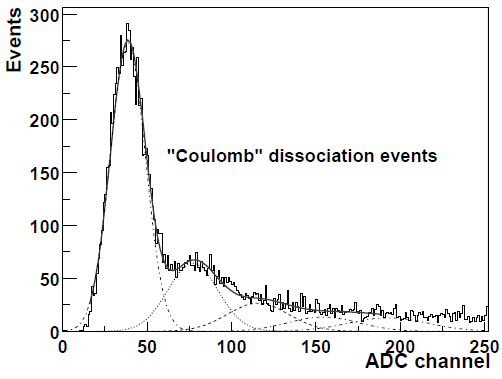
\includegraphics[width=.65\textwidth]{neuSpecRHIC}
      \caption{ZDC neutron spectrum at RHIC with each a Gaussian fit 
         to the 1, 2, 3, 5, and 5 neutron peak \cite{upcNeuPHENIX}.}
      \label{fig:neuSpecRHIC}
    \end{figure}
    Figure~\ref{fig:neuSpecRHIC} shows the charge recorded by the ZDCs (see Section~\ref{sec:zdcDet}).
    The peak at $\sim 30$ in Fig.~\ref{fig:neuSpecRHIC} is due to emission of a 
      single neutron. 
    Each successive peak is due to emission of an additional neutron. 
    From these peaks, the cross section for nuclear break-up by neutron 
      emission by both nuclei was measured.
    The fraction of nuclear interaction in all events with neutrons on both sides
      of the interaction point was found to be 0.661 $\pm$ 0.014 \cite{upcNeuPHENIX},
      which is in agreement the value 0.659 predicted by the model described in 
      \cite{emPCite4}.

    Nuclear collisions were separated from photon-induced break up by counting
      hits in the central scintillating counter similar to a tracker. 
    Events with hits on both sides of the interaction point were categorized as
      nuclear interactions, and those with no hits or hits on only one side were
      categorized as electromagnetic interactions. 
    The difference in the charge measured on each of the two sides of the 
      interaction point, by the two ZDCs, is divided by the total charge
      for both ZDCs (see Fig.~\ref{fig:neuRHICEMvHad}).
    \begin{figure}[!Hhbt]
      \centering
      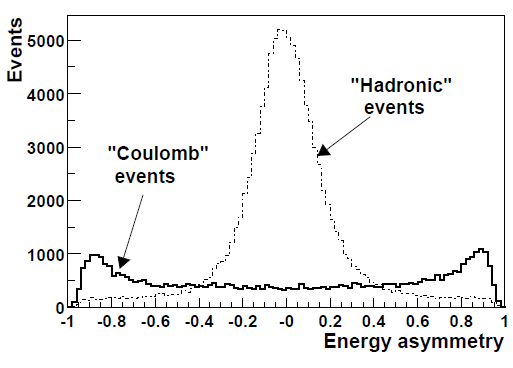
\includegraphics[width=.65\textwidth]{neuRHICEMvHad}
      \caption{The energy asymmetry in the ZDCs for photon-induced interaction, 
        coulomb events, and nuclear interaction, hadronic events \cite{upcNeuPHENIX}.}
      \label{fig:neuRHICEMvHad}
    \end{figure}
    Figure~\ref{fig:neuRHICEMvHad} shows that events created by electromagnetic 
      interactions result in asymmetric neutron emission, whereas nuclear 
      interactions produce neutrons on both sides. 
    In the analysis presented in this thesis, the energy asymmetry in the ZDCs is
      used to select UPC events.
    This will be discussed in Chapter~\ref{ch:trigg}.
    
    Both the $\rho^{0}$ and \JPsi{} meson photoproduction cross sections in UPC 
      events were measured at RHIC.
    STAR measured the photoproduction of the $\rho^{0}$ meson at collisions 
      energies per nucleon of 62.4 GeV \cite{upcRhoSTAR12}, 130 GeV 
      \cite{upcRhoSTAR02}, and 200 GeV \cite{upcRhoSTAR08}. 
    The \JPsi{} was measured by PHENIX at 200 GeV \cite{upcJPsiPHENIX}.
    The $\rho$ measurements by STAR were in good agreement with the theory
      calculation method described in Section~\ref{sec:vdmTheory}.
    The \JPsi{ } measurement where limited by statistic as only 10 \JPsi{}
      candidates were found. 

  \subsection{ UPC \JPsi{} at the LHC}
    The increase in beam energy from 200 GeV at RHIC to 2.76 TeV at the LHC 
      results in an increase in the Lorentz $\gamma$ of about 10.
    Because the photon flux depends on $\gamma^{2}$, the photon flux
      at the LHC increases by a factor of about 100 compared to RHIC.
    All major heavy ion experiments, ALICE and CMS, have studied the production
      of UPC events. 
    ALICE has studied coherent \JPsi{} photoproduction in ultra-peripheral PbPb
      collisions at $\sqrt{s_{NN}}$ = 2.76 TeV. 
   The cross section for this process was measured at both forward-rapidity, 
      $y$ = 3~\cite{Abelev:2012ba}, and mid-rapidity, $y$ = 0~\cite{Abbas:2013oua}.
   With an integrated luminosity of 55 $\mu$$b^{-1}$, ALICE measured 
     78 $\pm$ 10(stat) $^{+7}_{-11}$(syst) coherent \JPsi{} candidates at 
     forward rapidity.
   The measured cross section was 1.00 $\pm$ 0.18(stat) $_{-0.26}^{+0.24}$ 
    (syst) mb.
   For a symmetric system like PbPb collisions, as opposed to pPb collisions, 
    there is an ambiguity between which ion is the target and which is the 
    photon emitter. 
  Therefore, the cross section has a contribution from the low-$x$ and high-$x$ 
    parts of the gluon density. 
  At $y$ = 3  for PbPb collisions at the LHC, the cross section has a 
    contribution from both $x$ = 5 $\times 10^{-5}$ and $x$ = 2  $\times 
    10^{-2}$.
  This ambiguity is not present at $y$ = 0.
  ALICE has also measured the coherent \JPsi{} photoproduction cross section 
    at $y$ = 0, using a integrated luminosity of about 23 $\mu$$b^{-1}$.
  291 $\pm$ 18 (stat)$\pm$ 4(syst) and 265 $\pm$ 40 (stat)$\pm$ 12(syst) 
    coherent \JPsi{} candidates were measured in the dimuon and dielectron
    channels, respectively. 
  The combined cross section from both channels was measured to be 
    2.38 $_{-0.24}^{+0.34}$ (stat+syst) mb. 
  At $y$ = 0 $x$ $\sim$ 10$^{-3}$, which is a smaller $x$ than at forward 
    rapidity, and more sensitive to the nuclear gluon shadowing 
    (see Fig.~\ref{fig:aliceMoney}).
    \begin{figure}[!Hhbt]
      \centering
      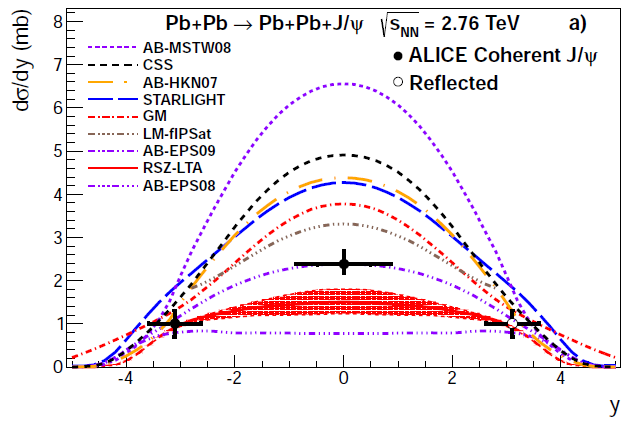
\includegraphics[width=.65\textwidth]{aliceJpsiCo}
      \caption{Coherent \JPsi{} photoproduction cross section in ultra-peripheral
        PbPb collisions at $\sqrt{s_{NN}}$ = 2.76 TeV, measured by the ALICE 
        experiment at forward and mid-rapidity~\cite{Abelev:2012ba,Abbas:2013oua}.}   
      \label{fig:aliceMoney}
    \end{figure}

    The ALICE data points have been compared to several theoretical models. 
  The UPC photoproduction cross section calculations depend significantly on 
    how the nucleus is represented in the calculation. 
  The results from the STARlight, LTA, and AB methods vary from a relatively 
    large cross section in the STARlight model, ranging through a variety of values
    in the AB method, to a relatively small cross section in the LTA method. 
  Each of these methods utilizes the same probe of the nucleus, the equivalent 
    photon flux that is calculated using the Weizs\"{a}cker-Williams approximation 
    (see Section~\ref{sec:wwAprox}). 
  The three methods deviate in how they calculate the forward photoproduction
    scattering cross section.
  The differences in the UPC photoproduction cross sections predicted by the 
    different models demonstrates the amount of experimental sensitivity there 
    is to distinguishing between the models. 
  The dependence of the cross section on rapidity is clearly visible.   

  The cross section value calculated by Eq.~\ref{eq:finalSTARlightResult} in the 
    STARlight, LTA, and the various gluon density models in AB method vary 
    significantly.
  Table~\ref{tab:allXsec} gives the predicted values for the three main methods
    taken from \cite{pQCD2013.02}, \cite{lta2011.09}, and \cite{vmd1999}.
  \begin{table} 
   \centering
   \begin{tabular}{|l|l|} 
     \hline
     Model & $\sigma_{AA\rightarrow AAJ/\psi} (mb)$ \\ \hline \hline
     STARlight/STARlight MC & 23 \\ \hline
     LTA & 9 \\ \hline
     AB-MSTW08 & 34 \\ \hline
     AB-EPS08 & 7  \\ \hline
     AB-EPS09 & 14 \\ \hline
     AB-HKN07 & 23 \\ \hline
     \hline
   \end{tabular}
   \caption{$\sigma_{AA\rightarrow AAJ/\psi} (mb)$
    the LTA, STARlight, AB methods. Four different gluon density models~\cite{pQCD2011.08,pQCD2013.02,Pumplin:2002vw} are used 
    in the AB method. STARlight is a simulation software package that utilizes 
    the STARlight model.}
   \label{tab:allXsec}
  \end{table}
  The cross sections in Table~\ref{tab:allXsec} differ by a factor of 4 
    from the smallest to largest and create an experimental opportunity. 
  The clear discrepancy between the models in Table~\ref{tab:allXsec} 
    demonstrates the high amount of experimental sensitivity there is for 
    distinguishing between the models. 

  The nuclear suppression factor, S, demonstrates the difference between how 
    the models represent the nucleus. 
  $S$ is the ratio between the nuclear photoproduction cross section and the     
    free nucleon photoproduction cross section.
  It is a measure of how the nuclear gluon densities evolve in each of the 
    models. 
  Figure.~\ref{fig:ltaAndPqcdNucSub} from \cite{lta2013.05} shows the nuclear 
    suppression, which is equivalent to $R_g$ in Eq.~\ref{eq:ltaOptTheWNucMo}, 
    for the LTA and AB methods.
  \begin{figure}[h] 
    \begin{center}
      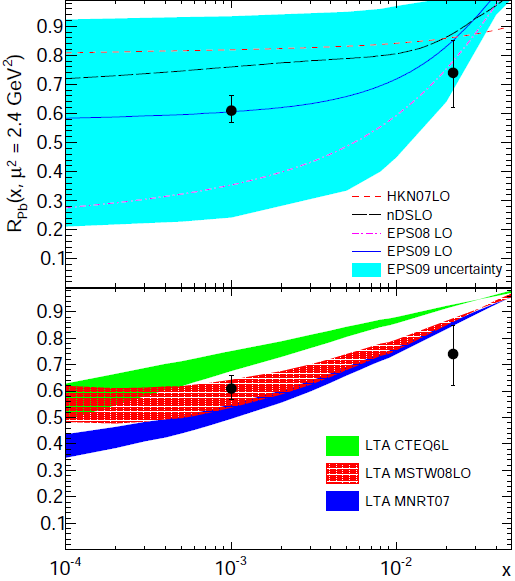
\includegraphics[width=0.5\textwidth,keepaspectratio]{ltaAndPqcdNucSub.png}
    \end{center}
    \caption{ \label{fig:ltaAndPqcdNucSub} Nuclear supression factor, $S$, in the AB and LTA methods~\cite{lta2013.05}.}
  \end{figure}
  \begin{figure}
    \begin{center}
      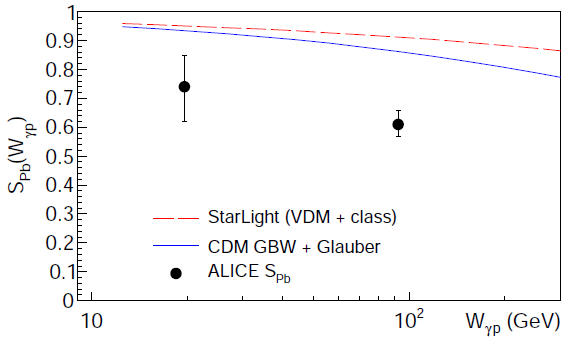
\includegraphics[width=0.5\textwidth,keepaspectratio]{ltaAndPqcdNucSubVMD.png}
    \end{center}
    \caption{ \label{fig:ltaAndPqcdNucSubSTARlight} Nuclear supression factor, $S$, in STARlight method~\cite{lta2013.05}.}
  \end{figure}
  Fig.~\ref{fig:ltaAndPqcdNucSubSTARlight} shows the nuclear suppression for the STARlight 
    method \cite{lta2013.05}. 
  Fig.~\ref{fig:ltaAndPqcdNucSub} and Fig.~\ref{fig:ltaAndPqcdNucSubSTARlight} 
    show that as the momentum of the probing photon goes up, increasing 
    $W_{\gamma p}$, and momentum of the probed gluon goes down, decreasing $x$, 
    the nuclear gluon density decreases relative to the free nucleon. 
  The nuclear suppression factor, $S$, allows for the different models' 
    representations of the gluon content of the nucleus to be directly compared
    to each other and to data. 
  $S$ can be measured from data by assuming a Weizs\"{a}cker-Williams photon flux and 
    provides insight into nuclear gluon densities.

  In addition, ALICE reported the measurement of the incoherent \JPsi{} 
    photoproduction cross section at mid-rapidity~\cite{Abbas:2013oua}.
  This provided additional constraints to the models for gluon shadowing. 

  In Chapter~\ref{ch:analysis}, the coherent UPC \JPsi{} photoproduction 
    cross section using CMS is described.
  The measurement in this thesis adds to existing ALICE results, covering
    an intermediate range of $x$ values. 
